\chapter{Модель мелкой воды как составная часть модели гидротермодинамики океана}\label{ch:ch1}

\section{Математическая постановка задачи}\label{sec:ch1/sec1}

Рассматриваемая в работе модель основана на системе нелинейных уравнений мелкой воды, которая записывается в произвольной ортогональной системе координат
в следующем виде:

\begin{equation} \label{eq:ch1/sec1/1}
    \begin{array}{c}
        \displaystyle{ \d{r_x r_y h u}{t} + T_u(u, v) - F_u(u, v) - h r_x r_y l v + r_y h g \d{\zeta}{x} = RHS_u } \\

        \displaystyle{ \d{r_x r_y h v}{t} + T_v(u, v) - F_v(u, v) + h r_x r_y l u + r_x h g \d{\zeta}{y} = RHS_v } \\

        \displaystyle{ \d{h}{t} + \frac{1}{r_x r_y} \left( \d{u r_y h}{x} + \d{v r_x h}{y} \right) = 0 }
    \end{array}
\end{equation}

Где $r_x, r_y$ - метрические коэффициенты Ламе, возникающие при записи системы уравнений в произвольной ортогональной системе координат;
$u$, $v$ – компоненты усредненного по глубине вектора горизонтальной скорости; $l$ – параметр Кориолиса;
$g$ – ускорение свободного падения; $\zeta$ – отклонение уровня моря относительно невозмущённого состояния;
$h = H + \zeta$ – полная глубина океана; $H$ – глубина океана в состоянии покоя.
Операторы переноса $T_u$ , $T_v$ записываются в криволинейной системе координат в дивергентной форме:
\begin{equation} \label{eq:ch1/sec1/2}
    \begin{array}{c}
        \displaystyle{T_{u} (u,v,h)=\frac{\partial hr_{y} uu}{\partial x} +\frac{\partial hr_{x} vu}{\partial y} - h\left(v\frac{\partial r_{y} }{\partial x} -u\frac{\partial r_{x} }{\partial y} \right)v} \\

        \displaystyle{T_{v} (u,v,h)=\frac{\partial hr_{y} uv}{\partial x} +\frac{\partial hr_{x} vv}{\partial y} + h\left(v\frac{\partial r_{y} }{\partial x} -u\frac{\partial r_{x} }{\partial y} \right)u}
    \end{array}
\end{equation}

Операторы вязкости $F_u$ , $F_v$ записываются как дивергенция тензора напряжений:
\begin{equation} \label{eq:ch1/sec1/3}
    \begin{array}{c}
        \displaystyle{F_{u} (u,v)=\frac{1}{r_{y} } \frac{\partial }{\partial x} \left(r_{y} ^{2} KD_{T} h\right)+\frac{1}{r_{x} } \frac{\partial }{\partial y} \left(r_{x} ^{2} KD_{S} h\right)} \\

        \displaystyle{F_{v} (u,v)=-\frac{1}{r_{x} } \frac{\partial }{\partial y} \left(r_{x} ^{2} KD_{T} h\right)+\frac{1}{r_{y} } \frac{\partial }{\partial x} \left(r_{y} ^{2} KD_{S} h\right)}
    \end{array}
\end{equation}

Здесь $\textit{K}$ - коэффициент вязкости, а $D_T$ и $D_S$ - компоненты тензоров напряжений сжатия-растяжения и сдвига соответственно:
\begin{equation} \label{eq:ch1/sec1/4}
    \begin{array}{c}
        \displaystyle{D_{T} =\frac{r_{y} }{r_{x} } \frac{\partial }{\partial x} \left(\frac{u}{r_{y} } \right)-\frac{r_{x} }{r_{y} } \frac{\partial }{\partial y} \left(\frac{v}{r_{x} } \right)} \\

        \displaystyle{D_{S} =\frac{r_{x} }{r_{y} } \frac{\partial }{\partial y} \left(\frac{u}{r_{x} } \right)+\frac{r_{y} }{r_{x} } \frac{\partial }{\partial x} \left(\frac{v}{r_{y} } \right)}
    \end{array}
\end{equation}

В общем случае в правых частях $RHS_u$ , $RHS_v$ рассчитываются градиенты атмосферного
давления и напряжения трения ветра. 
\begin{equation} \label{eq:ch1/sec1/5}
\begin{array}{c} 
\displaystyle{RHS_u = P_{x} + \tau _{x}^{surf}} \\ 

\displaystyle{RHS_v = P_{y} + \tau _{y}^{surf}} 
\end{array} 
\end{equation} 
Здесь $P_x, P_y$ - градиенты атмосферного давления на поверхности океана, $\tau^{surf}$ - напряжение силы ветра на поверхности.
В правых частях также могут рассчитываться и приливные силы,
рассчитываемые через приливной потенциал.

На берегах для скорости задаются граничные условия непротекания и свободного скольжения.

Именно в виде \cref{eq:ch1/sec1/1} - \cref{eq:ch1/sec1/4} нелинейные уравнения мелкой воды представлены в сигма модели общей циркуляции океана INMOM,
возникающие при разрешении быстрых баротропных гравитационных волн \cite{INMOM}, \cite{ChaplyginSW2017}.
Важно отметить, что все переменные в данной постановке задачи двумерные.
В противном случае правые части должны содержать интегралы по глубине от нелинейного взаимодействия трёхмерных величин, в частности, адвективных слагаемых.

\section{Описание численной реализации}\label{sec:ch1/sec2}

\subsection{Дискретизация по пространству}\label{sec:ch1/sec2-1}

Система уравнений \cref{eq:ch1/sec1/1} - \cref{eq:ch1/sec1/4} в модели разрешается с использованием численных методов.
При дискретизации по пространству нелинейных уравнений мелкой воды используется сетка в общем случае нерегулярная по долготе и широте.
Разобьём область $\{ x \in [x_0, x_{max}], \quad y \in [y_0, y_{max}] \}$, куда входит область, на которой рассматривается система уравнений \cref{eq:ch1/sec1/1},
на элементарные ячейки, которые будут иметь форму прямоугольников:

$$ \{ (x, y) : x_{m-1} < x < x_{m}, \quad y_{n-1} < y < y_{n} \} $$

Для решения системы уравнений \cref{eq:ch1/sec1/1} применяется техника построения разностных аппроксимаций по пространству второго порядка точности на разнесенной
'C'-сетке по классификации Аракавы \cite{ARAKAWA1976}, \cite{ARAKAWA1977}. На рис. \cref{fig:grid} показаны распределения переменных в каждой сеточной ячейке.
В центре ячейки задаются $\zeta$ и $H$. На серединах боковых сторон ячейки задаются
компоненты вектора скорости $(u, v)$ и потоковые переменные.
Параметр Кориолиса $l$ определяется в угловых точках.

\begin{figure}[htb!]
    \center
    \includegraphics[scale = 0.6]{CgridBig.png}
    \caption{Распределение переменных на ячейке модельной сетки}
    \label{fig:grid}
\end{figure}

При построении разностных схем особое место уделяется тому, чтобы
в разностных аналогах дифференциальных операторов сохранялись свойства симметрии,
которые выполняются для исходной дифференциальной задачи.
Это позволяет в разностной задаче автоматически удовлетворять энергетическим соотношениям, справедливым для дифференциальной.
Методика построения пространственных разностных аппроксимаций хорошо изложена, например, здесь \cite{ROUCH}, \cite{MARCHUK}.

\subsection{Дискретизация по времени}\label{sec:ch1/sec2-2}

При дискретизации нелинейных уравнений мелкой воды в качестве схемы по времени  используется схема 'Чехарда со средней точкой' ('leapfrog').
Для определения решения на шаге $n+1$ используются решения на шагах $n$ и $n-1$.

Рассмотрим простейшее уравнение адвекции:
\begin{equation} \label{eq:ch1/sec1/6}
    \frac{dU}{dt} = F(U)
\end{equation}
Применяя численную схему по времени 'Чехарда со средней точкой', получим следующее:
\begin{equation} \label{eq:ch1/sec1/7}
    \frac{U^{n+1} -U^{n-1} }{2\tau } = F(U^{n})
\end{equation}

У такой схемы по времени есть основной недостаток: расщепления решения по нечетным и четным временным шагам \cite{ROUCH}.
Поэтому на каждом временном шаге $n$ делается фильтрация \cite{POM}:
\begin{equation} \label{eq:ch1/sec1/8}
    U^{s} = U^{n} + \frac{a}{2}(U^{n+1} - 2U^n + U^{n-1})
\end{equation}
Затем, при переходе на следующий шаг по времени, $U^{s}$ присваивается $(n-1)$-му шагу, а решение $U^{n+1}$ присваивается $n$-му.
Параметр для фильтрации выбран как $a = 0.05$ \cite{POM}.

Для донного трения в системе уравнений \cref{eq:ch1/sec1/1} используется неявная схема Эйлера по времени,
что повышает устойчивость численного алгоритма.

\section{Тестирование модели мелкой воды}

%\subsection{Моделирование цунами в Японии}

\subsection{Моделирование экстремального шторма в Азовском море}

С помощью вышеописанной модели мелкой воды проводилось моделирование экстремального шторма на Азовском море, произошедшего 24 марта 2013 г.
Пространственное разрешение использованной модели составляло 250 метров,
атмосферные данные были взяты из расчетов по WRF (Weather Research and Forecasting
Model) из работы \cite{AzovStorm}. 
Моделирование проводилось на 3 месяца с шагом по времени 1 секунда, использовался коэффициент донного трения $n = 0.025$.
Было проведено сравнение с экспериментальными данными и сравнение результатов расчетов по нелинейным и линеаризованным уравнениям мелкой воды \cite{MARESEDU}.
Линейные уравнения мелкой воды представляют из себя упрощенную систему \ref{eq:ch1/sec1/1}:

\begin{equation} \label{eq:1linear} 
	\begin{array}{c} 
	\displaystyle{\frac{\partial r_{x} r_{y} u}{\partial t} - r_{x} r_{y} l v + r_{y} g\frac{\partial \zeta }{\partial x} + r_x r_y \frac{g n^2}{h^{1/3}} u \sqrt{u^2 + v^2}= 0} \\ 
	
	\displaystyle{\frac{\partial r_{x} r_{y} v}{\partial t} + r_{x} r_{y} l u  +r_{x} g\frac{\partial \zeta }{\partial y} + r_x r_y \frac{g n^2}{h^{1/3}} v \sqrt{u^2 + v^2}= 0} \\ 
	
	\displaystyle{\frac{\partial \zeta}{\partial t} +\frac{1}{r_{x} r_{y} } \left(\frac{\partial u r_{y} H}{\partial x} +\frac{\partial v r_{x} H}{\partial y} \right)= 0} 
	\end{array} 
\end{equation}
	
В такой модели используется предположение $h \approx H$ при $\zeta << H$.

\begin{figure}[htb!]
	\center
	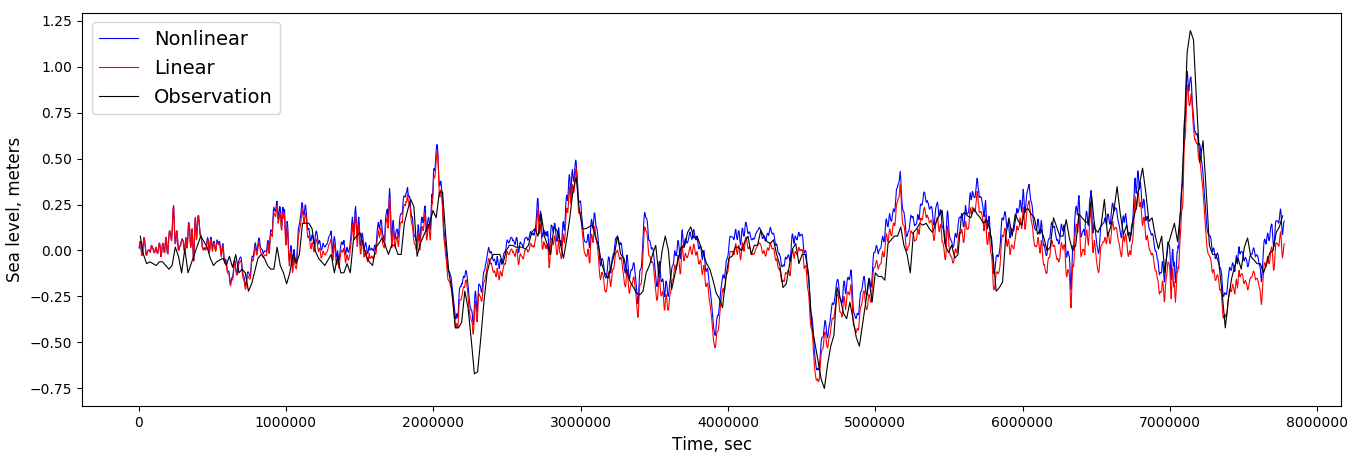
\includegraphics[width=0.85\linewidth]{EeskX.png}
	\caption{Моделирование шторма в акватории Азовского моря, сравнения уровня (метры) для поста "Ейск". 
		 Синий - нелинейные уравнения мелкой воды; красный - линеаризованные уравнения; черный - наблюдения}
	\label{fig:AS_Eesk}
\end{figure}
	
\begin{figure}[htb!]
	\center
	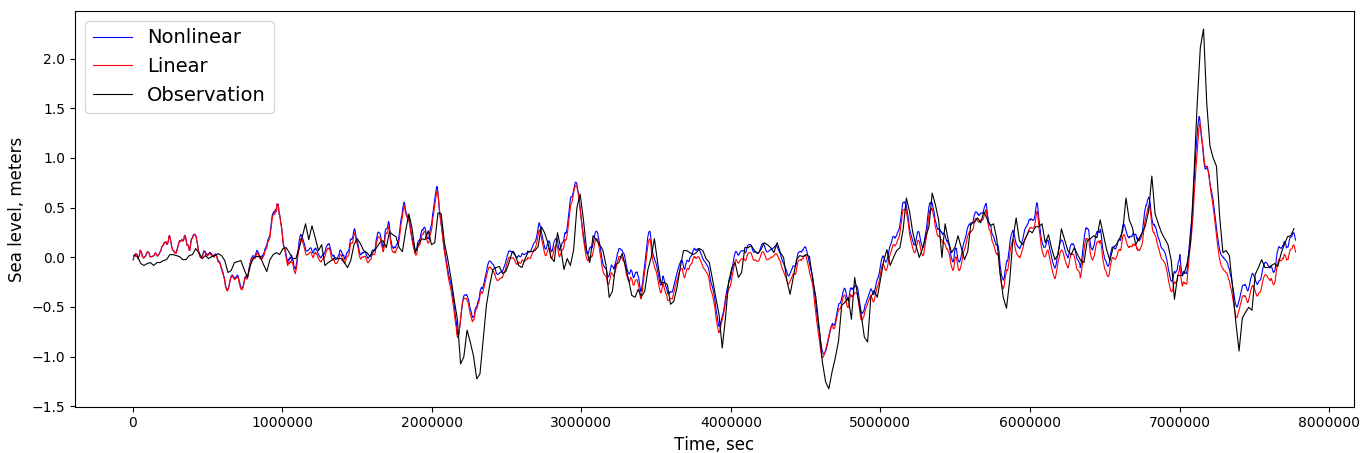
\includegraphics[width=0.85\linewidth]{TaganrogX.png}
	\caption{Моделирование шторма в акватории Азовского моря, сравнения уровня (метры) для поста "Таганрог". 
		 Синий - нелинейные уравнения мелкой воды; красный - линеаризованные уравнения; черный - наблюдения}
	\label{fig:AS_Taganrog}
\end{figure}

На рисунках \ref{fig:AS_Eesk}, \ref{fig:AS_Taganrog} продемонстрированы результаты расчетов (как по нелинейным уравнениям мелкой воды, так и по линеаризованным уравнениям) и данные наблюдений, полученные со станций "Ейск" и  "Таганрог" соответственно.
Из графиков видно, 
что результаты, полученные с помощью модели мелкой воды, хорошо согласуются с наблюдательными данными, и также было показано, что вклад нелинейности для этой задачи незначителен.

\FloatBarrier